\section*{Zadanie 19.}
\begin{task}
Zespolony wektor pola elektrycznego fali o $f=1 GHz$ rozchodzącej się w ośrodku stratnym, o parametrach: $\mu=\mu_{0} \ \epsilon=\epsilon_{0}$, oraz impedancji właściwej $Z=|Z|e^{j\cfrac{\pi}{18}}$ wyraża się zależnością: $\vec{E}=(\vec{i_{x}}+3j\vec{i_{y}})e^{j(\omega t - \beta z) - \alpha z} [\cfrac{V}{m}]$.
\begin{enumerate}[a)]
\item Zapisać odpowiadający mu wektor $\vec{H}$ w postaci rzeczywistej oraz narysować krzywą zakreślaną przez koniec tego wektora w płaszczyźnie $0xy\ (z=0)$
\item Obliczyć wartości $|Z|$, $\alpha$ oraz $\beta$. Podać wzór na zależność od czasu wartości powierzchniowej gęstości mocy tej fali w płaszczyźnie $z=2m$. 
\end{enumerate}
\textbf{Uwaga: Można wybrać (po uprzednim zaznaczeniu) łatwiejszą wersję zadania z założeniem
ośrodka bezstratnego (Z rzeczywiste, $\alpha=0$) z oceną maksymalną 10 p.}\\
\end{task}

\begin{solution}
$$\vec{E}=(\vec{i_{x}}+3j\vec{i_{y}})e^{j(\omega t - \beta z)- \alpha z}$$
$$\vec{E}(t)=\vec{i_{x}}e^{-\alpha z}\cos(\omega t - \beta z)-3\vec{i_{y}}e^{-\alpha z}sin(\omega t - \beta z)$$
$$\vec{H}=\cfrac{\vec{k}\times\vec{E}}{Z}$$
\begin{enumerate}[a)]
\item $$\vec{H}(t)=\vec{i_{y}}\cfrac{1}{|Z|}e^{-\alpha z}\cos{(\omega t - \beta z + Arg Z)+\cfrac{3}{|Z|}\vec{i_{x}}e^{-\alpha z}sin(\omega t - \beta z + Arg Z)}$$\\
Wartości liczbowe mogą się troche różnić, ale ogólny sens obrazka jest zachowany (9902 to liczba punktów dla których rysowany był wykres). Oczywiście elipsa powinna być wyciągnięta w górę, o czym mówią wartości, ale jak się narysowało każdy widzi.
\begin{center}
$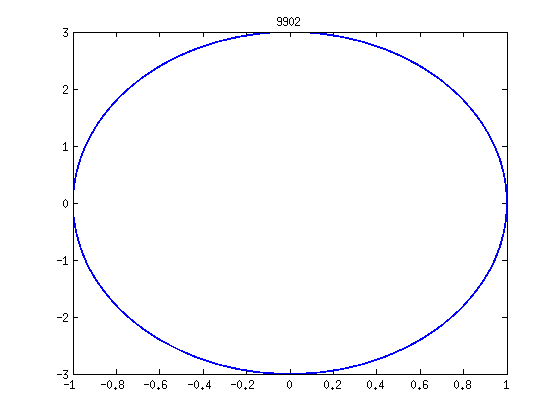
\includegraphics[scale=0.7]{19}$\\
\end{center}
\item $$Z=|Z|e^{j\cfrac{\pi}{18}}$$\\
$$Z=\sqrt{\cfrac{j\omega \mu}{\sigma + j\omega\epsilon}}=\sqrt{\cfrac{j\mu}{(\tg{\delta}+j)\epsilon}}=Z_{0}\sqrt{\cfrac{j}{\tg{\delta}+j}}$$
$$\delta = 2Arg Z\ \implies \delta = \cfrac{\pi}{9} \implies \tg{\delta}=0.35$$
$$|Z|=120\pi|\sqrt{\cfrac{j}{0.35+j}}|=365.7 \Omega$$
$$\gamma= \sqrt{j \omega\mu( \sigma+j \omega \epsilon)} = j \omega \sqrt{ \mu\eps} \big{(} 1 - j \cfrac{1}{2} \tg{ \delta}  \big{)} = 
2\cdot 10^{9}j\sqrt{\cfrac{1}{36\pi}\cdot 10^{-9}\cdot 4\pi\cdot 10^{-7}}\big{(} 1-\cfrac{1}{2}j\cdot 0.35 \big{)}=1.1(6)+ 6.(6)j$$\\
$\alpha=0.58(3) \ \cfrac{Np}{m}\\ \beta=3.(3)\ \cfrac{rad}{m} $\\
Wektor Poyntinga:
$$\vec{S}=\vec{E}\times\vec{H} =\cfrac{e^{-2\alpha x}}{|Z|} \begin{vmatrix}
					\vec{i_{x}}&\vec{i_{y}}&\vec{i_{z}}\\
					\cos{(\omega t-\beta z)}&-3\sin{(\omega t-\beta z+\cfrac{\pi}{18})}&0\\
					3\sin(\omega t - \beta z)&-\cos(\omega t - \beta z+\cfrac{\pi}{18})&0\end{vmatrix}=\cfrac{e^{-2\alpha x}}{|Z|} \big{(} \vec{i_{z}}\cos{(\omega t -\beta z)}\cos{(\omega t -\beta z + \cfrac{pi}{18})}+$$  $\ \ \ \ +\ \vec{i_{z}} 9\sin{(\omega t - \beta z)}\sin{(\omega t - \beta z+\cfrac{\pi}{18})} \big{)} $\\
$ \vec{S}(z=2m)=\cfrac{e^{-2.(3) x}}{365.7} \big{(} \vec{i_{z}}\cos{(2\cdot 10^{9} \pi t -13.(3))}\cos{(2\cdot 10^{9} \pi t -13.(3) + \cfrac{pi}{18})}+$\\ $\hspace{2.5cm} +\vec{i_{z}} 9\sin{(2\cdot 10^{9} \pi t - 13.(3))}\sin{(\omega t - 13.(3) +\cfrac{\pi}{18})} \big{)} $

\end{enumerate}
\end{solution}
